\begin{frame}{Etablering af søer}

\small

\begin{columns}[T]

\begin{column}{0.58\textwidth}

\textbf{Regler for etablering af søer:}

\begin{itemize}[]
\item Min. 600 m²
\item Minimum 10 m bufferzone
\item Min. 50\% af bufferzonen skal være soleksponeret
\item Pointgivende i 5 år fra anlæggelsestidspunktet
\end{itemize}

\vspace{0.4em}

\textbf{Gavner arter:}

\footnotesize
Vibe, engsnarreskade, dobbeltbekkasin, rødbenet klire, gul vipstjert, 
sanglærke, agerhøne, gråstrubet lappedykker, gråand, krikand, 
padder (frøer, tudser, salamandere), guldsmed, libeller, 
vilde bier (kant), humlebier, markmus, pindsvin, flagermus, 
musvåge, tårnfalk, rørhøg

\end{column}

\begin{column}{0.40\textwidth}
\centering
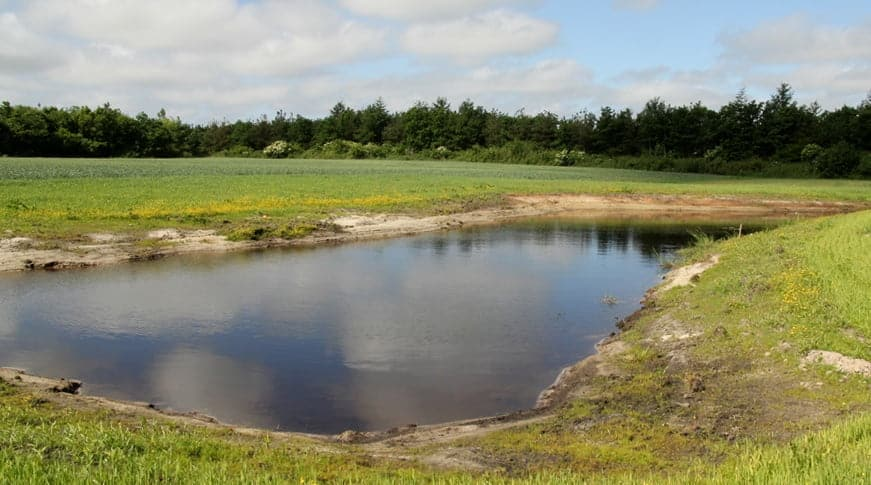
\includegraphics[width=\textwidth]{Billeder/Vildtforvaltning/biotopplantiltag/etableringafsø.jpg}
\end{column}

\end{columns}

\end{frame}